% TM - Data Structure
%%%%%%%%%%%%%%%%%%%%%%%%%%%%%%%%%%%%%%%%%%%%%

%%%%%%%%%%%%%%%%%%%%%%%%%%%%%%%%%%%%%%%%%%%%%%%%%%%%%%%%%%%%%%%%%%%%%%%%%

% EN
%\section{Implementation}

% FR
\section{Implémentation}

% EN
% In upcoming section following expressions will be used:

% \begin{tabular}{ll}
%   $n$ & number of nodes\\
%   $m$ & number of edges \\
%   $z$ & number of zones\\
%   $N$ & number of path computed for one pair of zone
% \end{tabular}

% Transportation modelling described in previous section was implemented in Python programming language using NumPy library.

% FR
Dans cette section, les expressions suivantes vont être utilisées :

\begin{tabular}{ll}
  $n$ & nombre de noeuds\\
  $m$ & nombre de bords \\
  $z$ & nombre de zone\\
  $N$ & nombre de chemin calculé pour une paire de zone
\end{tabular}

La modélisation de transport décrits dans la section précédente a été mise en œuvre dans le langage de programmation Python en utilisant la bibliothèque NumPy.

%%%%%%%%%%%%%%%%%%%%%%%%%%%%%%%%%%%%%%%%%%%%%%%%%%%%%%%%%%%%%%%%%%%%%%%%%

% EN
%\subsection{Static shortest path search}

% FR
\subsection{Recherche du plus court chemin statique}

% EN
% For determined $C$ we use Dijkstra's algorithm (complexity $O(m +n log(n) )$). So final complexity is 
% $$O(z (m + n log(n)))$$
% For traffic count we used also Dijkstra's algorithm. Final complexity for traffic count is 
% $$O(N z (m + n log(n)))$$
% For Dijkstra's algorithm we used Python library iGraph. iGraph is written in C programming language so it is quite fast. For example one Dijkstra running 30 ms ($n = 8000$ $m = 18000$).

% FR
Pour déterminer $C$ nous utilisons l'algorithme de Dijkstra's (de complexité $O(m +n log(n) )$). De fait, la complexité finale est de
$$O(z (m + n log(n)))$$
Pour le calcul du traffic nous avons aussi utilisé l'algorithme de Dijkstra. De fait, la complexité finale du calcul du traffic est de  
$$O(N z (m + n log(n)))$$
Pour l'algorithm de Dijkstra nous avons utilisé la bibliothèque Python iGraph. iGraph est écrit en C, c'est donc très rapide. Par exemple, un algorithme Dijkstra est exécuté en 30 ms ($n = 8000$ $m = 18000$).

%%%%%%%%%%%%%%%%%%%%%%%%%%%%%%%%%%%%%%%%%%%%%%%%%%%%%%%%%%%%%%%%%%%%%%%%%

% EN
%\subsection{Data store}

% FR
\subsection{Stockage des données}

% EN
% All data for transportation modelling are stored in relation database PostgreSQL with extension PostGIS. PostGIS is spatial extension. Using it you can manipulate with line, point, polygon, raster.

% FR
Toutes les données pour la modélisation des transports sont stockées dans une base de données PostgreSQL avec l'extension PostGIS. PostGIS est une extension spatiale pour les données géométrique. En l'utilisant, on pout manipuler les lignes, les points, les polygones, les annotations et les rasters.

% EN
% In database there are 6 main table:
% \begin{tabular}{|l|l|}
%   \hline
%   Table name & \\
%   \hline
%   \hline
%   \textbf{roads} & road links (edges)\\
%   \textbf{nodes} & nodes (vertexes)\\
%   \textbf{zones} & list of zones\\ 
%   \textbf{traffic} & \\
%   \textbf{general\_area\_information} & contains interested area geometry\\
%   \textbf{od\_pair} & Database implementation for $T$ matrix\\
%   \hline
% \end{tabular}

% FR 
Dans cette base de données on retrouve six tables principales :
\begin{tabular}{|l|l|}
  \hline
  Nom de table & Description \\
  \hline
  \hline
  \textbf{roads} & Les routes (edges)\\
  \textbf{nodes} & Les noeuds (vertexes)\\
  \textbf{zones} & La liste des zones\\ 
  \textbf{traffic} & \\
  \textbf{general\_area\_information} & l'aire géométrique contenant la zone d'intérêt\\
  \textbf{od\_pair} & Implémentation en base de données de la matrice $T$ \\
  \hline
\end{tabular}


% EN
% In Fig \ref{img.schema} there are all table in database model and relationships between them (arrow is FOREIGN KEY).

% FR 
La figure \ref{img.schema} schématise le modèle de la base de données avec les relations entre les tables.

\begin{figure}
  \centering
  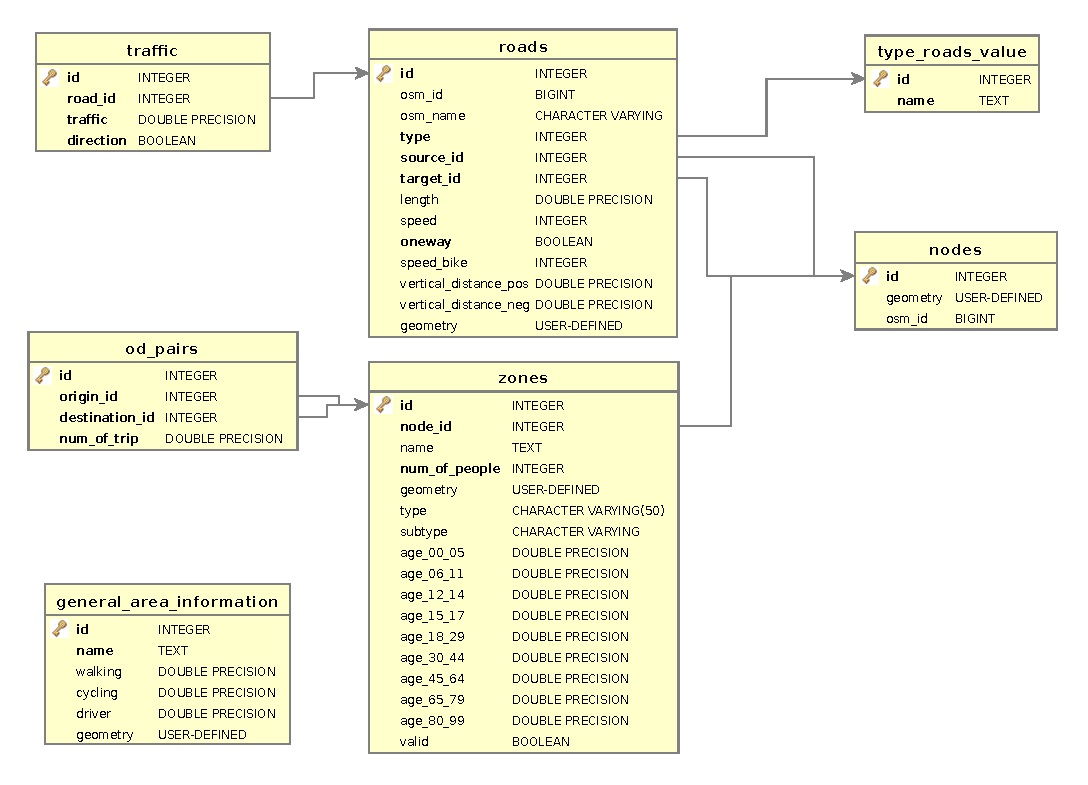
\includegraphics[width=15cm]{img/c01-transp-model/db.eps}
  \caption{Database model}
  \label{img.schema}
\end{figure}

% EN
% More details about DB you can find in project documentation on GitHub.

% FR
Plus de détails sont disponibles sur la documentation de notre dépot de code Github.

%%%%%%%%%%%%%%%%%%%%%%%%%%%%%%%%%%%%%%%%%%%%%%%%%%%%%%%%%%%%%%%%%%%%%%%%%

% EN
%\subsection{Future work}

% FR
\subsection{Prochains travaux}


% EN
%This method of transportation modelling is very hard ($O(N z (m + n log(n)))$), so it is suitable compute this problem in some parallel environment (shared (Threads) or distributed memory (MapReduce or MPI)).

% FR
Cette méthode de modélisation des transports est très difficile ($O(N z (m + n log(n)))$), il serait donc préférable d'adapter l'algorithme pour calculer ce problème dans un environnement parallèle (partagé par des threads, entre autre) ou de la mémoire distribuée (MapReduce ou MPI)).

